%\TEX root = ../../thesis_rui_almeida.tex
\section{Tomographic algorithms and reconstruction techniques}%
\label{sec:tomographic_algorithms_and_reconstruction_techniques}

\subsection{Introduction}%
\label{sub:tomography_introduction}

\todo[inline]{
    REPLACE
Tomography is the cross-sectional imaging of an object through the use
of transmitted or reflected waves, captured by the object exposure to
the waves from a set of known angles. It has many different applications
in science, industry, and most prominently, medicine. Since the
invention of the Computed Tomography (\gls{CT}) machine in 1972, by
Hounsfield~\cite{Gunderman2006}, tomographic imaging techniques have had
a revolutionary impact, allowing doctors to see inside their patients,
without having to subject them to more invasive
procedures~\cite{Kak2001}.

Mathematical basis for tomography were set by Johannes Radon in 1917. At
the time, he postulated that  it is possible to represent a function
written in $\mathbb{R}$ in the space of straight lines, $\mathbb{L}$
through the function's line integrals. A line integral is an integral in
which the function that is being integrated is evaluated along a curved
path, a line. In the tomographic case, these line integrals represent a
measurement on a ray that traverses the Region Of Interest (\gls{ROI}).
Each set of line integrals, characterized by an incidence angle, is
called a projection (see Figure~\ref{fig:projection} in
Section~\ref{sub:tomography}). To perform a tomographic reconstruction,
the machine must take many projections around the object. To the set of
projections arranged in matrix form by detector and projection angle, we
call sinogram. All reconstruction methods, analytical and iterative,
revolve around going from reality to sinogram to
image~\cite{Bruyant2002, Kak2001, Herman1973, Herman1995, Herman2009,
Defrise2003}.

There are two broad algorithm families when it comes to tomographic
reconstruction, regarding the physics of the problem. The problem can
involve either non-diffracting sources (light travels in straight
lines), such as the X-Rays in a conventional \gls{CT} exam; or
diffracting sources, such as micro-waves or ultrasound in more
research-oriented applications~\cite{Kak2001}. In this document, I will
not address the latter family, since I will not be applying them in my
work. In the next few paragraphs, I will discuss the first family of
algorithms, and describe how an image can be reconstructed from an
object's projections when the radiation source is non-diffracting.
}


Let's consider the case in which we deal with a single ray of solar
light entering the atmosphere at a given point. Since the atmosphere
contains numerous absorbers and comparable atmospheric effects, the ray
changes from the point where it enters the atmosphere to the point at
which it is measured by a detector. Total absorption will depend on the
pollutant species, their cross-section and their concentration, since it
obeys Lambert-Beer's law. Looking from another angle, this absorption
is also the line integral that we will use to reconstruct our image.
With \gls{DOAS}, it is possible to measure several pollutants at the
same time, but for simplicity (and since it is one of the most studied
compounds in the field), let's consider that the single pollutant in our
atmospheric mixture is NO$_2$.

\subsection{Initial Considerations}%
\label{sub:initial_considerations}

The problem of tomographic reconstruction can be approached in a number
of ways, depending mostly on the authors. In my literary search, I have
found that Kak and Slaney~\cite{Kak2001} have certainly explained this
problem in one of the clearer ways available. Therefore, I shall base
the rest of my presentation in their writings, and complement with other
authors' notes wherever necessary.

Considering the coordinate system displayed in
Figure~\ref{fig:coordinates}. In this schematic, the object is
represented by the function $f(x, y)$. The  $(\theta, t)$ parameters can
be used to define any line in this schematic. Line AB in particular can
be written:

\begin{equation}
    \label{eq:lineAB}
    x \cdot \cos(\theta) + y \cdot \sin(\theta) = t
\end{equation}

\begin{figure}[htpb]
    \centering
    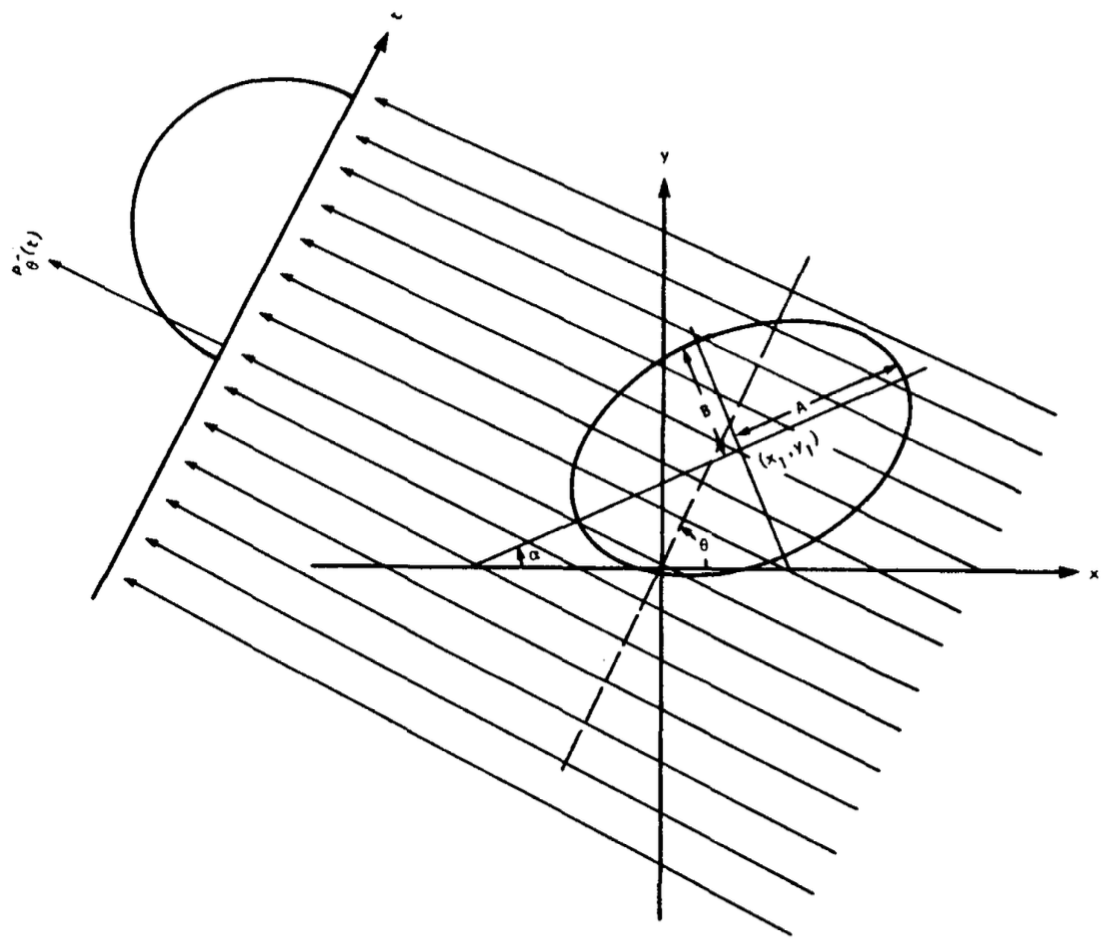
\includegraphics[width=0.7\textwidth]{img/png/coordinates.png}
    \caption{Schematic representation for coordinate setting. The image
    depicts a parallel projection setting~\cite{Kak2001a}.}
    \label{fig:coordinates}
\end{figure}

And if we were to write a line integral along this line, it would look
like Equation~\ref{eq:lineABIntegral}, the Radon transform of function
$f(x, y)$:

\begin{equation}
    \label{eq:lineABIntegral}
    P_{\theta}(t) = \int_{-\infty}^{\infty} f(x, y) \cdot \delta(x \cdot
    \cos(\theta) + y \cdot \sin(\theta) - t) dxdy
\end{equation}

Where $\delta$, the delta function, is defined in
Equation~\ref{eq:delta}.

\begin{equation}
    \label{eq:delta}
    \delta (\phi) =  
    \begin{cases}
            1, & \phi = 0\\
            0, & otherwise
    \end{cases}
\end{equation}

As I have mentioned previously, a projection is a set of line integrals
such as $P_{\theta}(t)$. Geometry plays a very important role in how the
integrals are written and solved for reconstruction. The simplest case
is the one where the set is acquired in a row, describing what is called
a parallel geometry. Another more complex case is when a single point
source is used as origin for all rays, forming a fan. This is called a
fan-beam array. There are other possible geometries, but they fall out of
the scope of this work and will therefore not be addressed any further.

\subsection{The Fourier Slice Theorem}%
\label{sub:the_fourier_slice_theorem}

The Fourier Slice Theorem (\gls{FST}) is the most important component of
the most important algorithm in tomographic inversion, the Filtered
BackProjection algorithm (\gls{FBP}). \gls{FST} is based on the equality
relation between the 
two-dimensional Fourier Transform (\gls{FT}) of the object function and
the one-dimensional \gls{FT} of the object's projection at an angle
$\theta$. Let's start by writing the 2D \gls{FT} for the object
function, Equation~\ref{eq:objectFT}, and the 1D \gls{FT} of projection
P$_\theta$, in Equation~\ref{eq:1dFTproj}.

\begin{equation}
    \label{eq:objectFT}
    F(u, v) = \int_{-\infty}^{\infty} \int_{-\infty}^{\infty} f(x, y)
    \cdot \exp \left [ -j2\pi (ux + vy) \right ] dx dy 
\end{equation}

\begin{equation}
    \label{eq:1dFTproj}
    S_{\theta}(\omega) = \int_{-\infty}^{\infty} P_{\theta} \cdot \exp\left[
    -j2 \pi \omega t \right]
\end{equation}

For simplicity, let's consider the 2D \gls{FT} at the line defined by
$v=0$ in the frequency domain. We rewrite the 2D \gls{FT} integral as:

\begin{equation}
    \label{eq:v0}
    F(u, 0) = \int_{-\infty}^{\infty} \int_{-\infty}^{\infty} f(x, y)
    \cdot \exp \left[  -j 2\pi  \omega ux \right] dx dy
\end{equation}

Notice that $y$ is not present in the phase factor of the \gls{FT}
expression anymore, and this means we can rearrange the integral as:

\begin{equation}
    \label{eq:v02}
    F(u, 0) = \int_{-\infty}^{\infty} \left[ \mathbf{\int_{-\infty}^{\infty}
    f(x, y) dy }\right] \cdot \exp \left[  -j 2\pi  \omega ux \right] dx 
\end{equation}

Now, the \textbf{bold} part of Equation~\ref{eq:v02} is similar to
Equation~\ref{eq:lineABIntegral}. It is precisely that equation,
considering $\theta=0$ and a constant value of $x$, as in
Equation~\ref{eq:p0}.

\begin{equation}
    \label{eq:p0}
    P_{\theta=0} (x) = \int_{-\infty}^{\infty} f(x, y) dy
\end{equation}

This in turn can be substituted in Equation~\ref{eq:v02}, finally
arriving at:

\begin{equation}
    \label{eq:FTP}
    F(u, 0) = \int_{-\infty}^{\infty} P_{\theta=0} (x) \cdot \exp \left[
    -j 2\pi ux \right] dx
\end{equation}

And this is the one-dimensional \gls{FT} for the projection at angle
$\theta=0$. Finally, the enunciation of the Fourier Slice Theorem:
\begin{center}
    \begin{minipage}{0.8\textwidth}

        \noindent\textbf{\emph{The Fourier Transform of a parallel
                projection  of an image $f(x, y)$ taken at angle
                $\theta$ gives a slice of the two-dimensional Fourier
                Transform, $F(u, v)$, subtending an angle $\theta$ with
                the $u$-axis (see Figure~\ref{fig:fst})}}

    \end{minipage}
\end{center}

\begin{figure}[htpb]
    \centering
    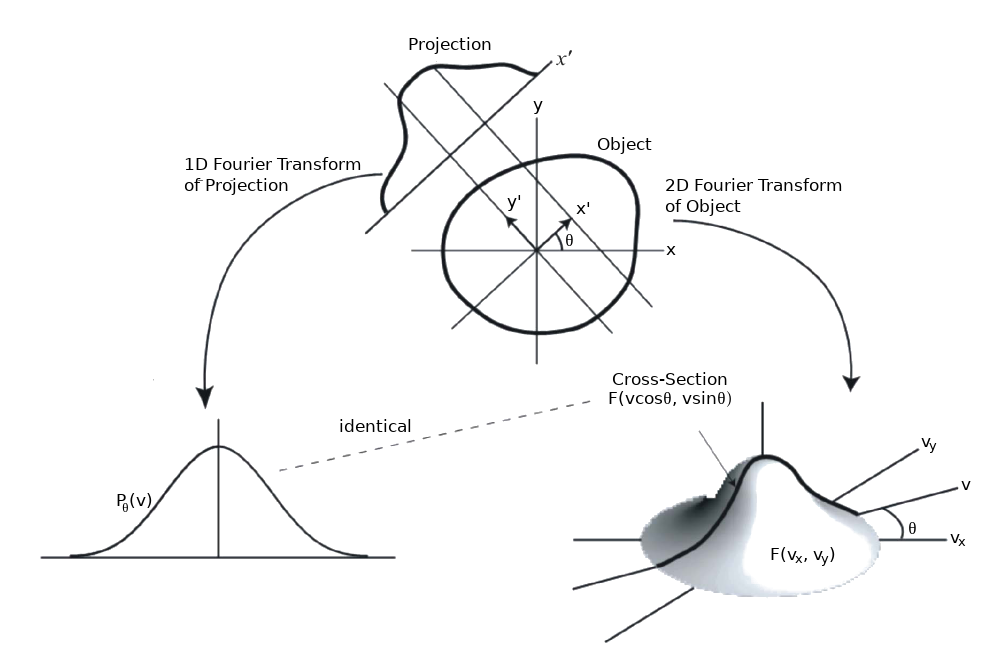
\includegraphics[width=.8\textwidth]{img/png/fst.png}
    \caption{The \gls{FST}, a schematic
    representation~\cite{Asl2013a}.}
    \label{fig:fst}
\end{figure}

\subsection{The Filtered BackProjection Algorithm}%
\label{sub:the_filtered_backprojection_algorithm}

\subsubsection{The rationale for \gls{FBP}}%
\label{ssub:the_rationale_for_fbp}

If one takes the \gls{FST} into account, the idea behind the \gls{FBP}
seems to appear almost naturally. Say one has a single projection and
its Fourier transform. From the \gls{FST}, this projection is the same
as the object's two-dimensional \gls{FT} in a single line. A crude
reconstruction of the original object would result if someone were to
place this projection in its right place in the Fourier domain and then
perform a two-dimensional \gls{IFT}, while assuming every other
projection to be 0. The result, in the image space, would be as if
someone had smeared the object in the projections direction.

What is really needed for a correct reconstruction is to do this many
times, with many projections. This brings a problem with the method:
smearing the object in all directions will clearly produce a wrong
\emph{accumulation} in the center of the image, since every projection
passes through the middle (remember we are still talking about parallel
geometry projections) and are summed on top of each other, but on the
outer edges, this does not occur. If one does not address this, the
image intensity levels in the reconstructed image will be severely
overestimated in the center and underestimated in the edges (due to
normalization). The solution is conceptually easy: we multiply the
Fourier transform by a weighting filter proportional to its frequency
($\omega$) and that encompasses its relevance in the global scheme of
projections. If there are $K$ projections, then it is adequate for this
value to be $\frac{2\pi\lvert\omega\rvert}{K}$. As an algorithm,
\gls{FBP} can be written as in Algorithm~\ref{alg:fbp}.

\begin{algorithm}
    \caption{The Filtered BackProjection Algorithm}
    \label{alg:fbp}
    \SetAlgoLined
    \KwResult{A reconstructed image of the projected object.}
    \For{$\theta \gets 0$ \KwTo $180$ \KwBy $\frac{180}{K}$}{
        measure projection $P_{theta}(t)$\;
        FT($P_{\theta}(t)$), rendering $S_{\theta}(\omega)$\;
        Multiply by $\frac{2\pi\lvert{\omega}\rvert}{K}$\;
        Sum the \gls{IFT} of the result in the image space\;
    }
    
\end{algorithm}


% \begin{algorithm}
%     \begin{algorithmic}
%         \FORALL{$\theta, \theta \in \left\{0..180,
%         \frac{180}{K}\right\}$}
%         \STATE{Measure projection $P_{\theta}(t)$;}
%         \STATE{FT($P_{\theta}(t)$), rendering $S_{\theta}(\omega)$}
%         \STATE{Multiply by $\frac{2\pi\lvert{\omega}\rvert}{K}$;}
%         \STATE{Sum the \gls{IFT} of the result in the image space.}
%     \ENDFOR
%     \end{algorithmic}
% \end{algorithm}

\subsubsection{Fan Projections Reconstruction}%
\label{ssub:fan_projections_reconstruction}

Parallel projections, in which the object is scanned linearly from
multiple directions, have the advantage of having a relatively simple
reconstruction scheme. However, they usually result in acquisition times
which are in the order of minutes. A faster way of collecting the data
is one where all radiation emanates from a single point-source, which
rotates around the target object (as well as the detectors). There are
two types of fan-beam projections: equiangular and equally spaced. In
this project, I have only worked with equiangular processes, so I will
not include an explanation for equally spaced fan-beam projections. The
reader may find this well described (much better than I would be able
to) in ~\cite{Kak2001} and ~\cite{Herman1973}.

Consider Figure~\ref{fig:equiangular}. If our projection data were
acquired through a parallel ray geometry, we would be able to say that
ray SA belonged to a projection $P_{\theta}(t)$, in which $\theta$ and
$t$ would be written:

\begin{equation}
    \label{eq:theta_and_t}
    \theta = \beta + \gamma \quad \text{ and } \quad t = D \cdot \sin \gamma
\end{equation}

In Equation~\ref{eq:theta_and_t}, $D$ is the distance between the source
$S$ and the origin $O$; $\gamma$ is the angle of a ray within a fan and
$\beta$ is the angle that the source $S$ makes with a reference axis.
Through these relationships one can \emph{translate} the parallel
projection's FBP algorithm to the fan-beam case, which involves several
complex geometric transformations, although the overall rationale is
exactly the same.

\begin{figure}[htpb]
    \centering
    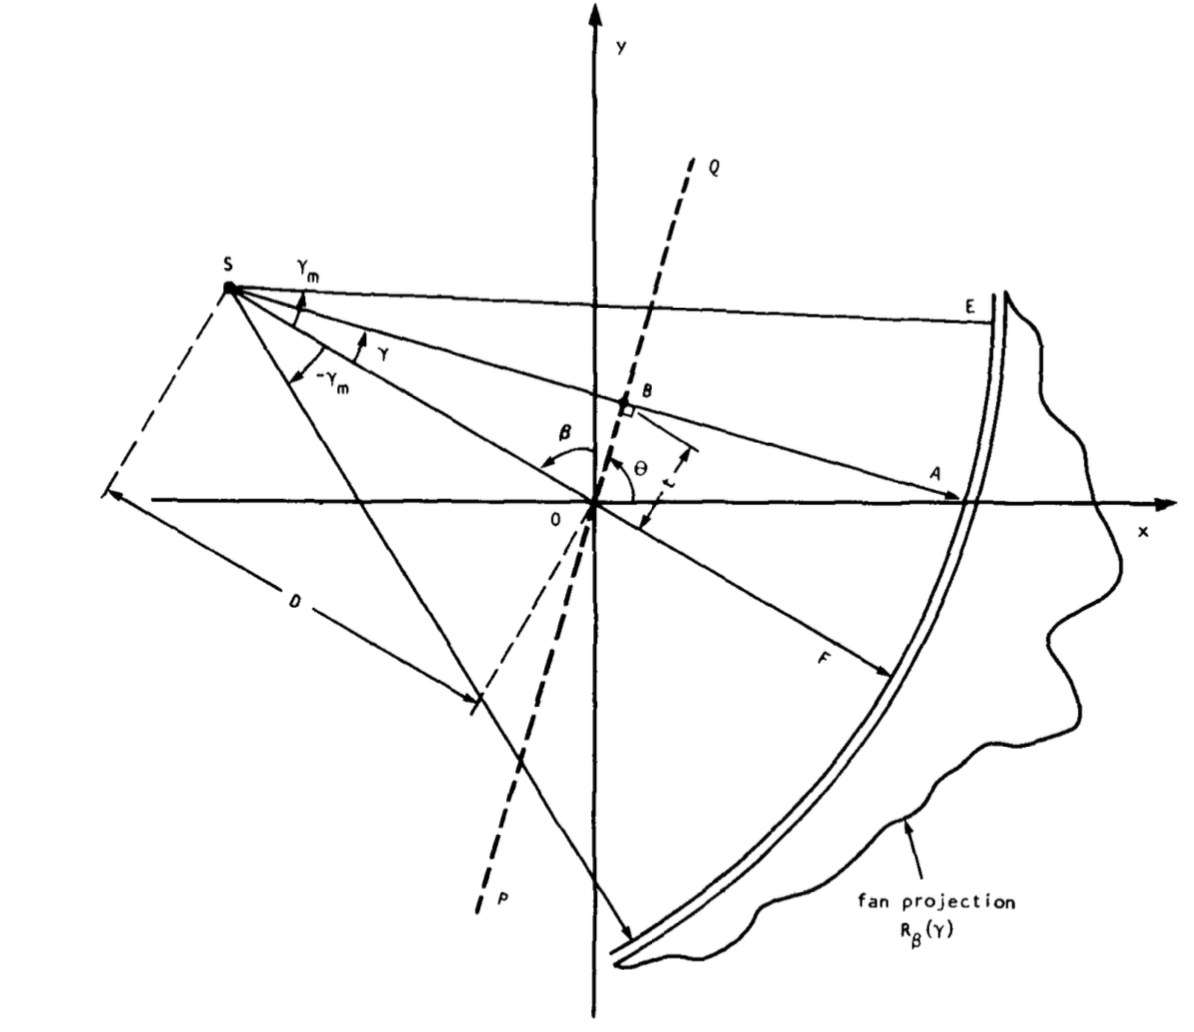
\includegraphics[width=.8\textwidth]{img/png/fig319.png}
    \caption{Schematic representation of an equiangular fan-beam
    projection, taken from~\cite{Kak2001}.}
    \label{fig:equiangular}
\end{figure}

Another particularity of fan-beam projection data is the fact that they
can be sorted into a parallel projection. For that, one starts with the
premise that if one were to substitute the fan geometry for parallel
beams, most of the fan-beam rays would also appear in some projection of
the parallel setup. This re-sorting algorithm starts with
Equation~\ref{eq:theta_and_t}. Now, if we call a fan-beam projection
taken at angle $\beta$ $R_{\beta}(\gamma)$, and a parallel projection
taken at angle $\theta$ $P_{\theta}(t)$, one could thus write
Equation~\ref{eq:parallel_vs_fanbeam}, which can already be used to
re-sort any fan-beam projection into parallel beam geometry.

\begin{equation}
    \label{eq:parallel_vs_fanbeam}
    R_{\beta}(\gamma) = P_{\beta + \gamma}(D \cdot \sin \gamma)
\end{equation}

Let's call the angular interval between fan-beam projections can be
written $\delta\beta$, and the angular interval of rays within each fan
is written $\delta\gamma$. In the case that they are the same
($\beta=\gamma=\alpha$), then it it is the case that they can both be
replaced by multiples of that interval in
Equation~\ref{eq:parallel_vs_fanbeam}, which becomes
Equation~\ref{eq:parallel_vs_fanbeam2}.

\begin{equation}
    \label{eq:parallel_vs_fanbeam2}
    R_{m \cdot \alpha}(n \cdot\alpha) = P_{m \cdot\alpha + n
    \cdot\alpha}(D \cdot \sin n \cdot\alpha)
\end{equation}

Or, in non-mathematical notation, the n\textsuperscript{th} ray of the
m\textsuperscript{th} radial projection (R) is the same as the
n\textsuperscript{th} ray in the (m+n)\textsuperscript{th} parallel
projection. Although being much simpler than directly applying the
\gls{FBP} algorithm to the fan-beam projection data, this method has a
limitation, which is the non-uniformity of the generated parallel
projections. This can usually be corrected through
interpolation~\cite{Kak2001a}. 
